\chapter{Reinforcement learning}

There are various RL algorithms. Here firstly we'll focus on Q learning.
\section{Q-learning}
\\
\begin{figure}
    \centering
    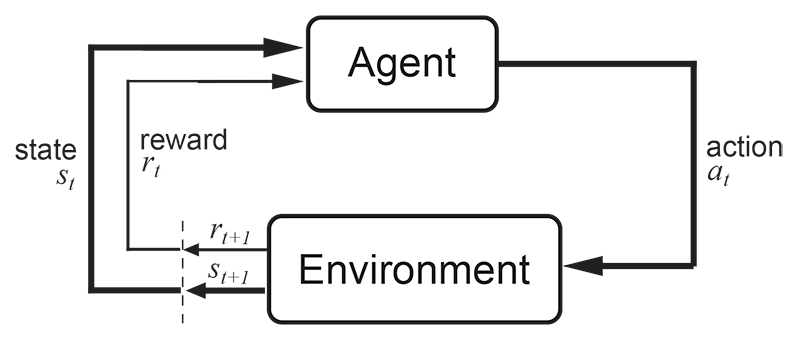
\includegraphics[width=\textwidth]{images/qlearn.png}
    \caption{Agent and environment}
\end{figure}
\\
\newline \textbf{Pseudo code}
\begin{figure}
    \centering
    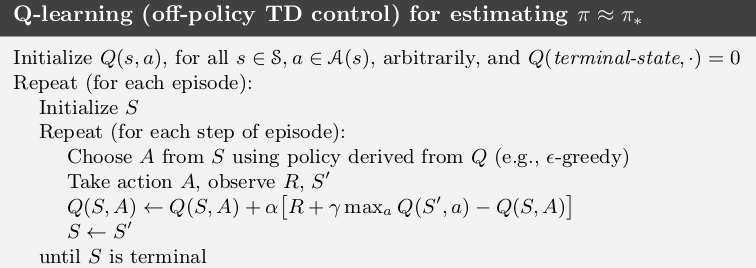
\includegraphics[width=\textwidth]{images/qlearnpseudo.png}
    % \caption{Mountain Car}
\end{figure}
\\
\section{OpenAI gym}
Openai gym is open source library for implementing the RL algorithm.
Let train the mountain car using the q learning as
\begin{figure}
    \centering
    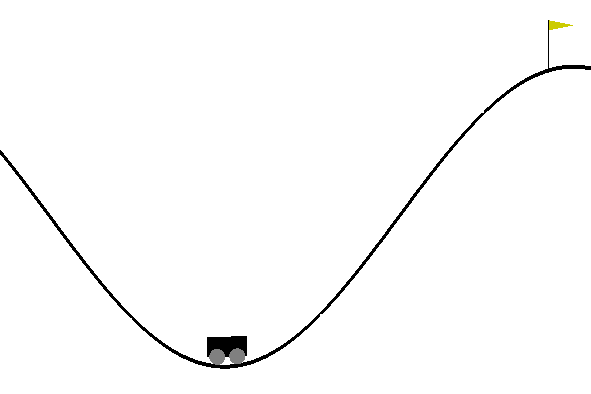
\includegraphics[width=0.5\textwidth]{images/mountaincar.png}
    \caption{Mountain Car}
\end{figure}
\\
\textbf{Code}
\begin{minted}{python}
'''
    Here variable are abreviated as,
    s - state
    sd - discretised state
    s_ - next state
    s_d - discretised next state
    ns - number of state
    a - action
    na - number of action
    Q - Q table
    rlist - list of reward
    avgrlist -  - list average of reward
    R - current reward
    ep - epsilon(exploration probability)
    mxep - max epsilon
    mnep - min epsilon
    epd - epsilon decay
    gamma - discount_rate
    lr - learning rate
    ne - number of episode
'''
#============== Import necessary libraries=================#
import numpy as np
import gym
import matplotlib.pyplot as plt
#========================== create env ===========================#
env = gym.make('MountainCar-v0')
env.reset()
#============== discretise state space=================#
def discret(temp):
    tempd = (temp- env.observation_space.low)*np.array([10, 100])
    tempd = np.round(tempd, 0).astype(int)
    return tempd
#============== value iteration =================#
def Viteration(env, lr, gamma, ep, mnep, ne):
    #=====ns=======#        !!! .n wont work
    ns = (env.observation_space.high - env.observation_space.low) * np.array([10, 100])#10 horzontal and 100 verticle
    ns = np.round(ns, 0).astype(int) + 1
    #=====qtable=======#
    Q = np.random.uniform(low = -1, high = 1, size = (ns[0], ns[1], env.action_space.n))
    #=====rsum, rlist, avgrlist=======#
    rlist = []
    avgrlist = []
    epd = (ep-mnep)/ne# Calculate episodic epd in ep
    #========== for ne episodes ============#
    for i in range(ne):
        done = False
        rsum,R = 0,0
        s = env.reset() #return (x,y)
        sd = discret(s)# Discretize
        #========== while not done ============#
        while done != True:
            if i >= (e - 20):# Render environment for last five e
                env.render()
            #====== explore vs exploit =====#
            if np.random.random() < 1 - ep:#epsilon greedy exr vs expt
                a = np.argmax(Q[sd[0], sd[1]]) 
            else:
                a = np.random.randint(0, env.action_space.n)
            s_, R, done, info = env.step(a) 
            s_d = discret(s_)# Discretize
            #====== update q =====#
            if done and s_[0] >= 0.5:#Allow for terminal states
                Q[sd[0], sd[1], a] = R
            else:# Adjust Q value for current s
                Q[sd[0], sd[1],a] =(1-lr)*Q[sd[0],sd[1],a]  +   lr*(R + gamma*np.max(Q[s_d[0], s_d[1]]))
            #====== variable update =====#
            rsum += R# Update variables
            sd = s_d
        #====== epsilion decay =====#
        if ep > mnep:# Decay ep
            ep -= epd
        rlist.append(rsum)# Track rewards
        #====== avg reward per 100 episodes =====#
        if (i+1) % 100 == 0:
            avgr = np.mean(rlist)
            avgrlist.append(avgr)
            rlist = []
            print('Episode {} Average Reward: {}'.format(i+1, avgr))
    env.close()
    return avgrlist
#===================== calling ================================#
lr=0.2
gamma=0.9
ep=0.8
ne=5000
mnep = 0
avgrlist = Viteration(env, lr, gamma, ep, mnep, e)
#========================= plot and save =========================#
plt.plot(100*(np.arange(len(avgrlist)) + 1), avgrlist)
plt.xlabel('Episodes')
plt.ylabel('Average Reward')
plt.title('Average Reward vs Episodes')
plt.savefig('rewards.jpg')
plt.show()
plt.close()
\end{minted}
\\
\newline \begin{figure}
    \centering
    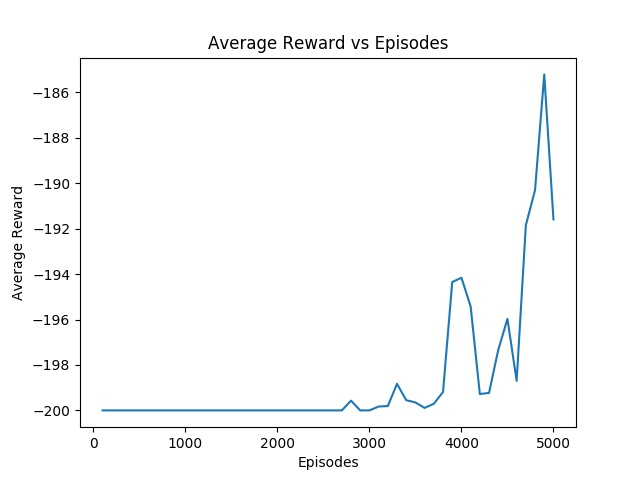
\includegraphics[width=0.8\textwidth]{images/rewards.jpg}
    \caption{Result - average reward for 100 episodes}
\end{figure}
\newline \\
\newline \section{Conclusion}
In this chapter, we studied the Q learning and implemented it on the mountain car problem using the openai gym library .

